\section{Systeme \skript{161}}	
	\subsection{Begriffe}
		\begin{tabularx}{\textwidth}{|p{4.5cm}|p{6cm}|X|}
		\hline
			\textbf{Bezeichnung}
		& 	\textbf{Beschreibung}
		& 	\textbf{Bedingung, Erkennung}
		\\ \hline
			Wirkungsfreiheit \skript{161}
		& 	Eingang des Systems hochohmig, \newline Ausgang niederohmig
		& 	Kaskadierte Systeme durch Einheitsverstärker verbunden
		\\ \hline
			Statische bzw. dynamische Systeme \skript{162}
		& 	Statisch: ohne Gedächtnis \newline 
			Dynamisch: mit Gedächtnis
		& 	Statisch: $u_2(t)$ nur vom Eingangssignal $u_1(t)$ bei $t$ abhängig \newline
			Dynamisch: $\int dt; \; \frac{d}{dt}; \; f(t \pm t_0) $
		\\ \hline
			Kausale bzw. akausale \newline Systeme \skript{164}
		& 	Kausal: Keine zukünftigen Werte \newline
			Akausal: System ''sieht in die Zukunft'' \newline
			\colorbox{yellow}{\parbox{6cm}{\textbf{Statische  und reale (physikalische) Systeme sind immer kausal!}}}
		& 	Kausal: $f(t - t_0); \int^t f(\tau) d \tau \quad (t_0 > 0)$ \newline
					$Impulsantwort:\ h(t) = 0 \ \ \forall \ t < 0 $ \newline \newline
			Akausal: $f(-t); \; f(t + t_0); \; \int^{t+t_0} f(\tau) d \tau$
		\\ \hline
			Lineare bzw. nichtlineare \newline Systeme \skript{165}
		&	Linear: Ausgangssignal hat keine \newline neuen Frequenzanteile \newline	
		Nichtlinear: Ausgangssignal kann \newline \textbf{neue Frequenzanteile}  enthalten
		& 	\textbf{Linear:} $S(x1+x2)=S(x1)+S(x2)$ \newline
		$S(c\cdot x)=c\cdot S(x)$, Superposition \newline
		\textbf{Nichtlinear:} $f^{\alpha}(t); \; \alpha + f(t); \; \alpha^{x(t)} $ \newline
			\textbf{$\Longrightarrow$ Kennlinie nicht durch Ursprung}	
		\\ \hline
			Zeitinvariante bzw. zeitvariante Systeme \skript{170}
		& 	Zeitvariant: Von der Zeit abhängig \newline
			Zeitinvariant: Von der Zeit unabhängig
		& 	Zeitvariant: $\cos(t) x(t); t^{\alpha} x(t) \quad \text{(} \alpha \neq 0 \text{)} $ \newline
			Zeitinvariant: $S(x(t-t_0)=S(x)\cdot x(t-t_0)$
		\\ \hline 
		\end{tabularx}
		
		
		\subsubsection{Beispiele \skript{118}}

			\bgroup
			\setlength{\tabcolsep}{1.3mm}
			\begin{tabularx}{\textwidth}{|c|c|c|l|l|X|}
			\hline
				\multicolumn{3}{|c|}{\textbf{Systemtyp}}
			&	\textbf{Mathem. Form}
			&	\textbf{Beispiel (kausal)}
			&	\textbf{Beispiel (akausal)}
			\\ \hline
				statisch
			&	linear
			&	zeitinvariant
			&	$y(t) = \gamma \cdot x(t)$
			&	$y(t) = 3 \cdot x(t)$
			&	
			\\ \hline
				statisch
			&	linear
			&	zeitvariant
			&	$y(t) = \gamma(t) \cdot x(t)$
			&	$y(t) = t^2 \cdot x(t)$
			&	
			\\ \hline
				statisch
			&	nichtlinear
			&	zeitinvariant
			&	$y(t) = f \left\lbrace  x(t) \right\rbrace $
			&	$y(t) = 4 \cdot x^2(t)$
			&	
			\\ \hline
				statisch
			&	nichtlinear
			&	zeitvariant
			&	$y(t) = f \left\lbrace  x(t),t \right\rbrace $
			&	$y(t) = t \cdot x^3(t)$
			&	
			\\ \hline
				dynamisch
			&	linear
			&	zeitinvariant
			&	
			&	$y(t) = \dfrac{d^2 x(t)}{d t^2} - \dfrac{2 dx(t)}{dt}$
			&	$y(t) = \dfrac{d^2 x(t+1)}{d t^2} - \dfrac{2 dx(t)}{dt}$
			\\ \hline
				dynamisch
			&	linear
			&	zeitvariant
			&	
			&	$y(t) = cos(t) \cdot \int\limits_{-\infty}^{t} x(\tau) d\tau $
			&	$y(t) = cos(t) \cdot \int\limits_{-\infty}^{t+1} x(\tau) d\tau $
			\\ \hline
				dynamisch
			&	nichtlinear
			&	zeitinvariant
			&	
			&	$y(t) = \dfrac{d^2 x(t)}{d t^2} - \dfrac{2 dx(t)}{dt} + 1$
			&	$y(t) = \dfrac{d^2 x(t+1)}{d t^2} - \dfrac{2 dx(t)}{dt} + 1$
			\\ \hline
				dynamisch
			&	nichtlinear
			&	zeitvariant
			&	
			&	$ \ddot y(t) = cos(t) \cdot x(t-1) - 0.5$
			&	$ \ddot y(t) = cos(t) \cdot x(t+1) - 0.5$
			\\ \hline
			\end{tabularx}
			\egroup
			
			
	\subsubsection{Linearisierung von Systemen: Siehe \skript{169}}

	\subsection{Übertragungsfunktion von LTI-Systemen \skript{174}}
		\begin{tabular}{ll}
			\parbox{13cm}{
				$$h(t) \; \laplace \; H(s)$$
				$$s_2(t) = h(t) * s_1(t) \; \laplace \; S_2(s) = H(s) S_1(s)$$}
		& 	\parbox{5cm}{
				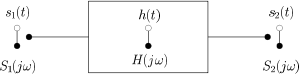
\includegraphics[width=5cm]{./bilder/utf-theorie.png}}
		\\
			\multicolumn{2}{l}{Kaskadierung von wirkungsfreien Systemen:
				$H_{total}(s) = H_1(s) H_2(s)$ bzw. bei $n$ gleichen Systemen:
				$H_{total} = (H(s))^n$}
		\\
		\end{tabular}
		
		\begin{tabular}{ll}
			\parbox{13cm}{ \beispiel{ \parbox{12cm}{
				\textbf{Beispiel}: Gesucht UTF $H(s) = \frac{Y(s)}{X(s)}$ \\
				$$H(s) = \frac{sL}{\frac{1}{sC} + sL + R} = \frac{s^2}{\frac{1}{LC} + s
					\frac{R}{L} + s^2}$$\\
				$$\Longrightarrow \text{Pole bei } s = -\frac{R}{2L} \pm j
				\sqrt{\frac{1}{LC} - \left(\frac{R}{2L}\right)^2} \quad ; \quad \text{Doppelte
				Nullstelle bei } s = 0$$
				Differentialgleichung:    $ \ddot{y}(t)+
				\frac{R}{L}\dot{y}(t)+\frac{1}{LC}y=\ddot{x}(t)$
			}}}
		& 	\parbox{5cm}{
				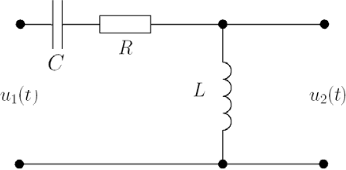
\includegraphics[width=5cm]{./bilder/utf-beispiel.png}}
		\\	
		\end{tabular}
		
		\subsubsection{Bestimmung der UTF}
		\parbox{10cm}{
			\begin{tabular}{ll}
				Bauteil & Ersatz \\
				R & R\\
				L & sL\\
				C & $\frac{1}{sC}$ \\
			\end{tabular}
			Parallelschaltung $= \frac{1}{\frac{1}{R}+\frac{1}{sL}+sC}$\\ \\
		}
		\parbox{8cm}{
			
			Das Potential in einem Punkt berechnet man mit $=\frac{Summe\ aller\
			Elemente\ zwischen\ Punkt\ und\ GND}{Summe\ aller\ Elemente\ der\ Kompletten\ Schaltung}$\\
			Die \textbf{Ordnung der UTF} ist die Anzahl unabhängiger Speicher (L oder C).}		
		
		\subsubsection{Asymptotische Steilheit}
			\parbox{9cm}{
			Die asymptotische Steilheit lässt sich aus der UTF bestimmen. 
			Folgende Schritte sind vonnöten:
			\begin{itemize}
				\item Den Amplitudengang von der UTF bestimmen.
				\item Den Summand mit der höchsten Ordnung von $\omega$ extrahieren/isolieren.
				\item Die Funktion ohne Faktor ist die Steilheit.
			\end{itemize}
			}
			\parbox{1cm}{
				\quad
			}
			\parbox{9cm}{
				\textbf{Beispiel:} \\
				$H(s) = \frac{sL}{s^3L^2C + s^2RLC} \rightarrow |H(\omega)|_{\omega >> 1} = \frac{sL}{s^3L^2C} = \frac{1}{L^2C}$
				\formel{$\frac{1}{\omega^2}$}
			}
		
			\paragraph{Steilheit in dB/Dekade}
				\parbox{5cm}{
					\formel{$H(\omega = 10) = 20 \cdot lg(f(\omega))$}
				}
				\parbox{4cm}{
					Die Funktion wird mit der dB-Formel berechnet und als Argument wird die Zahl 10 eingefügt. \\
				}
				\parbox{1cm}{
					\quad
				}
				\parbox{10cm}{
					\textbf{Beispiel:}	\\
					$H(s) = \frac{sL}{s^3L^2C + s^2RLC} \rightarrow |H(\omega)|_{\omega >> 1} = \frac{sL}{s^3L^2C} = \frac{1}{L^2C} \frac{1}{\omega^2}$	\\[5pt]
					\formel{$|H(\omega = 10)|_{dB} = 20 \cdot lg(\frac{1}{\omega^2})$} $= -40 dB/Dekade$
				}
		
		\subsubsection{Beispiele von Übertragungsfunktionen (verschiedene Filter)}
		\renewcommand{\arraystretchOriginal}{1}
		\begin{tabularx}{\textwidth}{|X|c|c|c|c|}
			\hline
			{}
			&	Tiefpassfilter
			&	Hochpassfilter
			&	Bandpassfilter
			&	Allpassfilter
			\\
			{}
			&	1. Ordnung
			&	1. Ordnung
			&	2. Ordnung
			&	1. Ordnung
			\\ \hline
			{}
			&	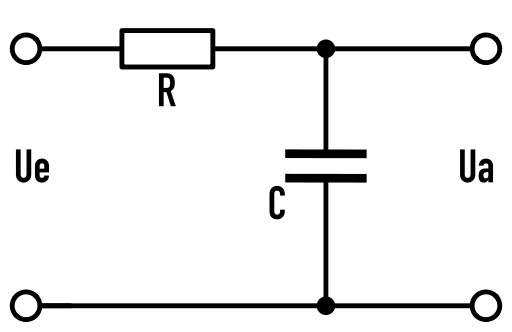
\includegraphics[width=2.5cm]{./bilder/tiefpass.png}
			&	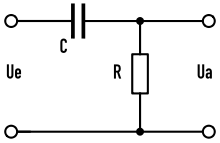
\includegraphics[width=2.5cm]{./bilder/hochpass.png}
			&	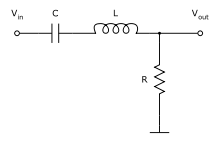
\includegraphics[width=2.5cm]{./bilder/bandpass.png}
			&	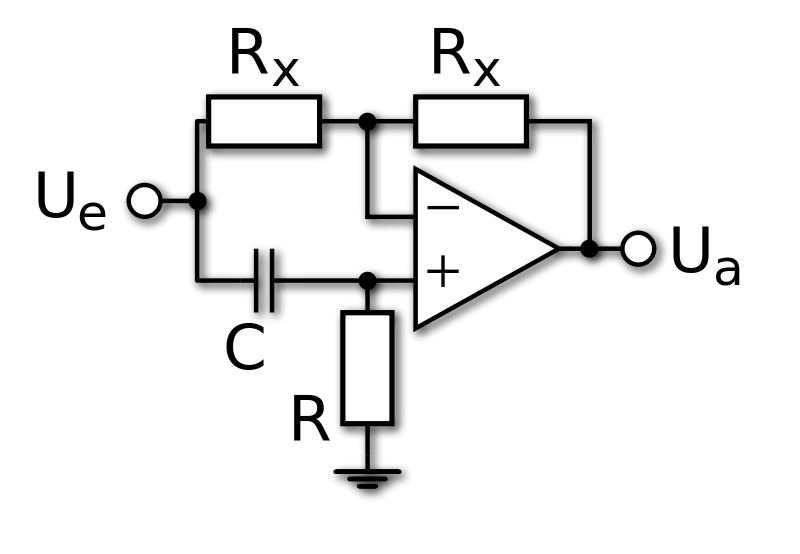
\includegraphics[width=2.5cm]{./bilder/allpass.png}
			\\ \hline & & & & \\
			Übertragungsfunktion $H(s)$
			&	$\dfrac{1}{1 + sRC}$
			&	$\dfrac{sRC}{1 + sRC}$
			&	$\dfrac{sRC}{1 + sRC + s^2 LC}$
			&	$\dfrac{sRC - 1}{sRC + 1}$
			\\ & & & & \\ \hline & & & & \\
			Amplitudengang $|H(\omega)|$
			&	$\dfrac{1}{\sqrt{1 + (\omega RC)^2}}$
			&	$\dfrac{|\omega RC|}{\sqrt{1 + (\omega RC)^2}}$
			&	$\dfrac{|\omega RC|}{\sqrt{(\omega^2 LC - 1)^2 + (\omega RC)^2}}$
			&	$1$
			\\ & & & & \\ \hline & & & & \\
			Phasengang $\varphi(\omega)$
			&	$-arctan(\omega RC)$
			&	$arctan(\dfrac{1}{\omega RC})$
			&	$-arctan(\dfrac{\omega^2 LC -1}{\omega RC})$
			&	$\pi - 2 arctan(\omega RC)$
			\\ & & & & \\ \hline & & & & \\
			Grenzfrequenz $f_c$
			&	$\dfrac{1}{2 \pi RC}$
			&	$\dfrac{1}{2 \pi RC}$
			&
			& 	
			\\ & & & & \\ \hline
			Spannung am Ausgang
			&	\multicolumn{4}{|c|}{
				$\text{Spannung am Eingang} \cdot |H(\omega)|$
			}
			\\ \hline
		\end{tabularx}
		
		\subsubsection{Berechnung des Amplituden- und Phasengangs aus der Übertragungsfunktion}
			
			$$H(j \omega) = \frac{Y(j \omega)}{X(j \omega)} = \underbrace{|H(j
			\omega)|}_{Amplitudengang} e^{j\overbrace{\Theta(\omega)}^{Phasengang}} = 
			\frac{|Y(j \omega)|}{|X(j \omega)|} e^{j (\arg(Y(j \omega)) - \arg(X(j
			\omega)))} =
			\frac{|Y(j \omega)|}{|X(j \omega)|} e^{j \left[\arctan \left(\frac{\Imag\{Y(j
			\omega)\}}{\Real\{Y(j \omega)\}} \right) - \arctan \left(\frac{\Imag\{X(j
			\omega)\}}{\Real\{X(j \omega)\}} \right)\right]}$$
			
			\begin{tabular}{ll}
				\textbf{Phasengang:} & 
				$\Theta(\omega) = \arctan \left(\frac{\Imag (H(j\omega))}{\Real (H(j\omega))}\right) \nonumber$ \\
				\textbf{Amplitudengang:} &
				$|H(j\omega)| = \frac{|Y(j\omega)|}{|F(j\omega)|} \nonumber$
			\end{tabular}
		
		
		\subsubsection{Zusammenhang zwischen Impuls- \& Einheitssprungantwort, Endwerte \skript{175}}
		
			$ \text{Einheitssprungantwort } g(t) \text{, Impulsantwort }h(t)$
			$$h(t)= \frac{d g(t)}{d t}\quad\text{bzw.}\quad
			g(t)=\int_{-\infty}^{t}h(\tau)d\tau \qquad;\qquad 
			\lim\limits_{t \rightarrow \infty}  h(t)= \lim\limits_{s \rightarrow 0} s H(s)
			\qquad;\qquad
			\lim\limits_{t \rightarrow \infty}  g(t)= \lim\limits_{s \rightarrow 0} H(s)$$
		
		
		\subsubsection{Zusammenhang zwischen Impulsantwort und Kausalität eines Systems \skript{176}}
		
			Damit ein System kausal ist, muss dessen Impulsantwort $h(t)$ für alle $t < 0$ gleich Null sein.\\
			\formel{$h(t) = 0 \ \ \forall \ t < 0 \ \ \Longrightarrow $ System kausal!}
			
	\subsection{Stabilität von LTI-Systemen \skript{177}}
		\renewcommand{\arraystretchOriginal}{1}
		\subsubsection{BIBO-Stabilität \skript{177}}
			\textit{BIBO = Bounded Input Bounded Output}\\
					Ein beliebiges System ist \textbf{BIBO-stabil}, wenn auf jedes \textbf{beschränkte Eingangssignal}
					das \textbf{Ausgangssignal} ebenfalls \textbf{beschränkt} ist.$|u_{in}(t)| < A \rightarrow |u_{out}(t)| < B$ mit $0 < A,B \in \mathbf{N} < \infty$
%	\begin{equation}
%		\int\limits_{-\infty}^{\infty} |h(t)| dt < \infty \nonumber
%	\end{equation}
		
	\subsubsection{Asymptotische Stabilität \skript{178}}
		
			\begin{tabular}{ll}
				Stabil: 
			& 	$\lim\limits_{t\rightarrow\infty} h(t) = 0$ \qquad Pole \textbf{nur} in der linken s-Halbebene.
				\textbf{Achtung: Nur \underline{Pole}, nicht \underline{Nullstellen}!!}
			\\
				Instabil: 
			& 	Mind. ein Pol in der rechten s-Halbebene oder mind. ein \textbf{mehrfacher} Pol auf der $j$-Achse der s-Ebene.
			\\
				Grenzstabil:
			& 	mindestens ein \textbf{einfacher Pol} (aber kein mehrfacher) auf der $j$-Achse, keine Pole rechts der $j$-Achse
			\end{tabular}
		
		
		\subsubsection{Stabilität mit Hurwitz-Polynom \skript{179}}
		
			Es wird jeweils das Polynom im \textbf{Nenner der Übertragungsfunktion} betrachtet:
$P(s) = a_n s^n + a_{n-1} s^{n-1} +\ldots +a_1s + a_0$ \\
Ist ein solches Polynom ein Hurwitz-Polynom, so ist das System \textbf{asymptotisch stabil}.
Handelt es sich um ein \textbf{modifiziertes Hurwitz-Polynom} so ergibt es ein
\textbf{grenzstabiles} System.\\ \\
$P(s)$ ist nur dann ein Hurwitz-Polynom, wenn folgende Bedingungen erfüllt sind:
\begin{enumerate}
	\item	alle Koeffizienten $a_i$ von $P(s)$ sind grösser als Null (und sind vorhanden).\\
				(bis zum und mit Polynomen von Grad 2, ist es notwendig, dass alle Koeffizienten positiv
				sind, damit das Polynom asymptotisch stabil ist)
	\item	alle Hurwitz-Determinanten $D_1$ bis $D_n$ sind grösser als Null\\
				\begin{align}
					D_1 &= a_{n-1} > 0 \nonumber\\
					D_2 &= \left|
						\begin{matrix}
							a_{n-1} & a_n\\
							a_{n-3} & a_{n-2}
						\end{matrix}\right| > 0 \nonumber \\
						&\vdots \nonumber \\
					D_{n-1} &= \left|
						\begin{matrix}
							a_{n-1} & a_n & 0 & 0 & \cdots & 0 \\
							a_{n-3} & a_{n-2} & a_{n-1} & a_n & 0 & 0 \\
							a_{n-5} & a_{n-4} & a_{n-3} & a_{n-2} & \cdots & 0 \\
							\vdots & \vdots & \vdots & \vdots & \ddots & 0 \\
							0 & 0 & 0 & \vdots & 0 & a_1
						\end{matrix}\right| > 0 \nonumber \\
					D_n &= a_0D_{n-1} > 0 \nonumber
				\end{align}
\end{enumerate}

\textbf{Modifiziertes Hurwitz-Polynom}\\
Nebst allen $a_i \geq 0$ müssen alle Hurwitz-Determinanten $D_1, D_2, \ldots, D_{n-2} > 0$
und $D_{n-1} = D_n = 0$ sein. \\ \\

Für Polynome $P(s) = a_n \cdot s^n + a_{n-1} \cdot s^{n-1} + \ldots + a_1 \cdot s^1 + a_0$ vom
Grad n gilt für $a_i > 0$:\\
\begin{tabular}{|l||l| l|}\hline
$N$   &   $P(s)$ ist ein Hurwitz-Polynom (stabil) &  $P(s)$ ist ein
modifiziertes Hurwitz-Polynom (grenzstabil) \\ \hline\hline
      1     &      gilt f"ur alle $P(s)$          &  $a_0=0$ \\ \hline
      2     &     gilt f"ur alle $P(s)$           &  $a_1=0$ \\ \hline
      3     &     $a_1a_2>a_0a_3$      &  $a_1a_2=a_0a_3$ \\ \hline
      4     &     $a_3(a_1a_2-a_0a_3)>a_1^2a_4$   &    $a_3(a_1a_2-a_0a_3)=a_1^2a_4$\\ \hline

      5    &     {\footnotesize $a_3a_4>a_2a_5$  und}   &     {\footnotesize $a_3a_4>a_2a_5$} \\
           &     {\footnotesize
           $(a_1a_2-a_0a_3)(a_3a_4-a_2a_5)>(a_1a_4-a_0a_5)^2$}   &  
           {\footnotesize $(a_1a_2-a_0a_3)(a_3a_4-a_2a_5)=(a_1a_4-a_0a_5)^2$} 
           
           	\\ \hline   
           			\end{tabular}\\
					
			\begin{itemize}
				\item Wenn \textbf{mindestens ein Koeffizient negativ} ist $(a_x < 0)$, dann ist das System \textbf{instabil}.
			  	\item Wenn \textbf{alle Koeffizienten negativ} sind, kann $-1$ ausgeklammert werden und in den Zähler verschoben werden\\
			  			$\Rightarrow$ \textbf{System stabil} oder \textbf{grenzstabil} %(siehe Punkt 3)
			  	\item Wenn \textbf{ein Koeffizient nicht vorhanden} ist $(a_x = 0)$, dann ist das System evtl. grenzstabil, 
			  			d.h. es ist eine \textbf{Überprüfung mit modifiziertem Hurwitz-Polynom} nötig.
			\end{itemize}

	\subsection{Phasen- \& Gruppenlaufzeit \skript{182}}
	
		\definecolor{gruppe}{rgb}{1,.75,0} % 255,192,0
		\definecolor{phase}{rgb}{1,0,0} % 255,0,0
		Die \textcolor{phase}{Phasenlaufzeit}  ist nur für reine Sinussignale bestimmbar: $\tau_P(\omega)=\frac{-\theta(\omega)}{\omega}$ \\
		Die \textcolor{gruppe}{Gruppenlaufzeit} hingegen ist für sämtliche Signale möglich: $\tau_G(\omega)=\frac{-d\theta(\omega)}{d\omega}$ \\
		\begin{center}
			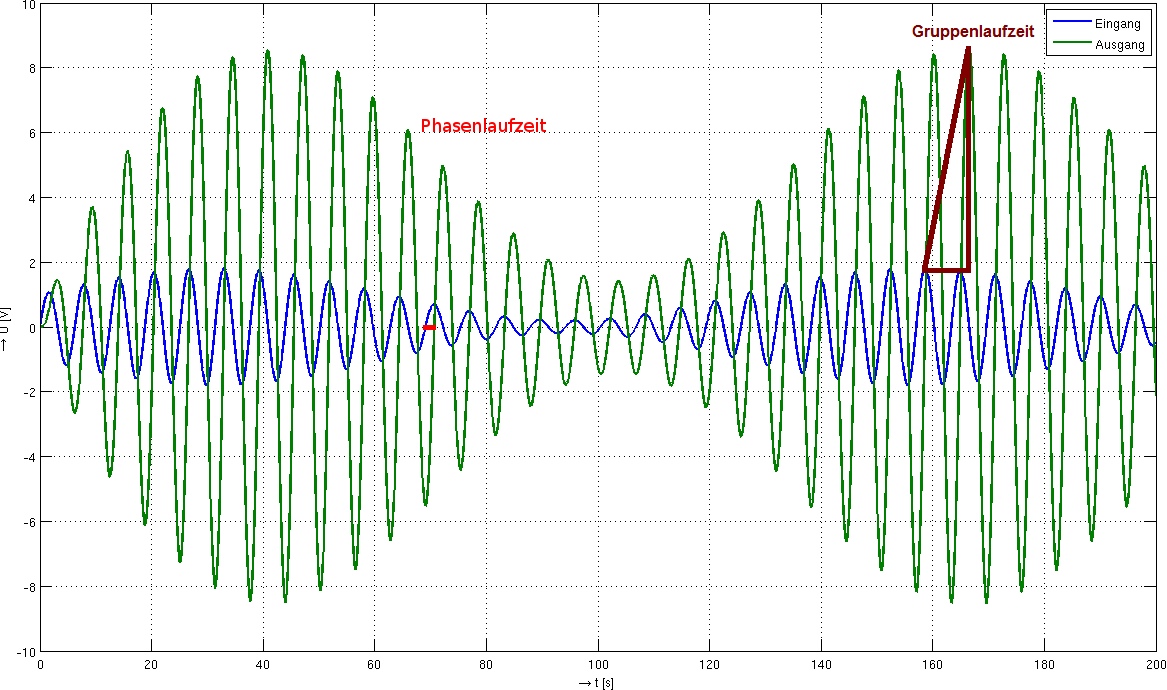
\includegraphics[width=14.5cm]{./bilder/laufzeit.png}
		\end{center}
		Eingangssignal $x(t)$ und Ausgangssignal $y(t)$ des Systems
		$H(s)=\frac{1}{s^2+0.2s+1}$. Bemerkung: $y(t)$ ist gr"osser als $x(t)$.
		
		
		\subsubsection{Signalverzögerung, Phasen- und Gruppenlaufzeit \skript{186}}
		
			Die \textbf{Signalverzögerung}, \textbf{Phasenlaufzeit} $\tau_P(\omega)$
			und \textbf{Gruppenlaufzeit} $\tau_G(\omega)$ sind identisch, wenn:
			\begin{itemize}
				\item \formel{$\theta(\omega) = -\omega \cdot t_0$}
				\item und der Amplitudengang ebenfalls konstant ist
			\end{itemize}
			
			Das heisst, $H(j \omega)$ hat die Form \formel{$H(j\omega) = a \cdot \e^{-j\omega t_0}$}. \\
			Die Signalverzögerung beträgt dann für alle Frequenzen \fbox{$t_0 = \tau_G = \tau_P$}.
		
	\subsection{Verzerrungen und Klirrfaktor \skript{187}}
		\subsubsection{Verzerrungen \skript{187}}
			\begin{tabular}{ll}
				\textbf{Lineare Verzerrungen:}
			&	\textbf{Nichtlineare Verzerrungen:}
			\\
				\parbox{9cm}{
					\begin{itemize}
						\item Erzeugen keine neuen Frequenzen
						\item z.B. Dämpfung (auch einzelner Frequenzen)
					\end{itemize}}
			&	\parbox{9cm}{
					\begin{itemize}
						\item Erzeugen neue Frequenzen
						\item z.B. Diode, Übersteuern, nichtlineare Kennlinien
					\end{itemize}}
			\\
			\end{tabular}
			
		\subsubsection{Masse für Verzerrung \skript{189}}
			Jedes verzerrte Signal kann durch ein Gütemass beschrieben werden. \\
			Diese sind:
			\begin{itemize}
				\item \textbf{Klirrfaktor:} Dieser stellt das Verhältnis des Effektivwertes der entstandenen Harmonischen und des Effektivwertes des gesamten Ausgangssignals. Dieses Mass wird insbesondere in Europa verwendet.
				\item \textbf{Total Harmonic Distortion (THD):} Dieser stellt das Verhältnis des Effektivwertes der entstandenen Harmonischen und des Effektivwertes der Grundschwingung. Dieses Mass wird insbesondere in USA verwendet. 
			\end{itemize}
			\begin{multicols}{2}
				\begin{description}
					\item Effektivwert des gesamten Ausgangssignal: 
					\item Effektivwert der entstandenen Harmonischen: 
					\item Effektivwert der Grundschwingung: 
					\item Effektivwert m-ten Harmonischen: 
				\end{description}
				\columnbreak
				\begin{description}
					\item $\sqrt{U_1^2 + U_2^2 + U_3^2 + ... + U_n^2}$
					\item $\sqrt{U_2^2 + U_3^2 + ... + U_n^2}$
					\item $U_1^2$
					\item $U_m^2$
				\end{description}
			\end{multicols}
		
			\paragraph{Klirrfaktor \skript{189}}
				\begin{tabularx}{\textwidth}{cX}
					\parbox{9cm}{
						Als Mass für nichtlineare Verzerrungen gilt der \textit{Klirrfaktor}. Betrachtet wird jeweils der Effektivwert am Ausgang.
						\begin{center}
							\formel{$k = \sqrt{\frac{U_2^2 + U_3^2 + \ldots + U_n^2}{U_1^2 + U_2^2 + \ldots + U_n^2}} $} $ 0 \leq k \leq 1$ 
						\end{center}
					}
						&	\parbox{9cm}{
						\begin{tabular}{ll}
							Teilklirrfaktor (frequenzselektiv):
						&	\fbox{$k_m =  \frac {U_m} {\sqrt{ U_1^2+ U_2^2 + \ldots + U_n^2} }$}
						\\
							Klirrdämpfungsmass:
						& 	\fbox{$a_k = 20 \log \left( \frac1k \right)$}
						\\
							Teilklirrdämpfungmass:
						& 	\fbox{$a_k = 20 \log \left( \frac{1}{k_m} \right)$}
						\end{tabular}
					}
				\end{tabularx}
			
			\paragraph{Total Harmonic Distortion (THD) \skript{189}}
				\begin{center}
					\fbox{$\text{THD} = \sqrt{ \frac {U_2^2+ U_3^2 + \ldots + U_n^2} {U_1^2} }$}
					$\infty > \text{THD} \geq k \geq 0; \quad \text{Für kleine Verzerrungen: THD} \approx k $
				\end{center}

		\subsection{Verzerrungsfreie Übertragung von Signalen \skript{190}}
		
			\begin{tabularx}{\textwidth}{p{9cm}X}
				Für eine Übertragung ohne Amplitudenverzerrung \newline (konstante Amplitude über alle Frequenzen) muss gelten:
			&	$ $ \newline \fbox{$|H(j\omega)| = konstant$}
			\\
			Für eine Übertragung ohne Phasenverzerrung \newline (Phase proportional zur Frequenz) muss gelten:
			&	$ $ \newline \fbox{$\theta(\omega) = -\omega t_0$}
			\end{tabularx}\\
			\\ \\
			Für eine \textbf{verzerrungsfreie Signalübertragung} müssen \textbf{beide Kriterien} erfüllt sein!\\
			\textbf{Dann gilt:}
			\begin{itemize}
				\item \fbox{$y(t) = a \cdot x(t-t_0) \ \; \laplace \; \ Y(j\omega) = a \cdot X(j\omega) \cdot \e^{-j\omega t_0}$}
				\item \fbox{$H(j\omega) = a \cdot \e^{-j\omega t_0} = |H(j\omega)| \cdot \e^{j \theta(\omega)} \ \Laplace \ h(t) = a \cdot \delta(t-t_0)$}
			\end{itemize}	
		
	\subsection{Übertragung von stochastischen Signalen \skript{193}}
		\begin{itemize}
			\item Linearer Mittelwert und Autokorrelationsfunktion des Ausgangssignales \skript{193}
			\item Leistungsdichtespektrum \skript{193}
			\item Kreuzkorrelationen \skript{194}
			\item \textbf{Beispiel:} Leistungsdichtespektrum am Ausgang eines RC-Tiefpasses \skript{195}
		\end{itemize}
		
		
		
		
		
		
		